{\let\clearpage\relax\let\cleardoublepage\relax
\chapter{Sistema solare}
}


\begin{workout}[Sistema solare - andamento densit\'a e composizione]
asteroid mercury mars mass depletion pg 298
\end{workout}

\begin{workout}[et\'a corpi sistema solare (age and chronology)]
helioseismology and meteoritic dating
\end{workout}


\begin{workout}[Struttura interna]
pg 256: interior and atmosphere, 293 solar system, 143 properties of transit
\end{workout}

\begin{workout}[Degree of super-adiabaticity: Struttura interna (assimption for pre-runaway accretion)]
See: characterization of exoplanets from their formation (pg4)
Degree of super-adiabaticity: baraffe 02, Rafikof 07
\end{workout}

\begin{workout}[few well separeted homogeneous region: Struttura interna (assimption for pre-runaway accretion)]
See: characterization of exoplanets from their formation (pg4)
Baraffe 07: composition gradients, core dissolution: Wilson, Militzer 12, planetesimal deconstruction: mordasini 05, multiconvective layers: Leconte chabrier 12.
\end{workout}

\begin{workout}[Full packing/spacing]

\end{workout}

\begin{workout}[Modello pianeta gassoso: Giove]

\end{workout}

\begin{workout}[Migrazione II: realistica]\end{workout}
grand tack (produce dinamical shack up) 
eccesso pianeti gioviani a 1au in simulazioni??
\begin{workout}[Noble gas enrichment]

\end{workout}


\begin{workout}[Orbit of terrestrial planets]
Constrain for core accretion model ofgiant planets: dynamical shakeup Nagasawa 05 Thommes08c
\end{workout}

\begin{workout}[Earth post-oligarchic growth]
perryman pg229
\end{workout}


\begin{workout}[Planetesima migration: pluto eccentricity, large population of Kuiper belt object]

\end{workout}



\begin{workout}[Planet obliquity:]
Schlichting sari 07: The effect of Semi-Collisional Accretion on Planetary Spins
Inconsistent with isotropic distro (Tremaine 1991). Randomly directed component of spin angular momentum (Kokubo Ida 07) cause large then observed i,e (Harris Ward 82).
Planetesimal/protoplanet collision would imply stachastic rather than smooth accretion.
Excittion of giant planet spin obliquity if spin axis precession freq pass through resonance with orbital prec freq during migration.
Uranus: tilt due to collision or migration: Bergstralh 91 or Bou\'e Laskar 10.
Non of obliquity of terrestrial planet are belived primordial (secular orbit perturbation)+tidal dissipation.
Effects of inhomogenous infall on obliquity (tremaine 91, bate 10)
\end{workout}



{\let\clearpage\relax\let\cleardoublepage\relax
\chapter{Alcune caratteristiche della popolazione di esopianeti}
}

La popolazione degli esopianeti osservata riflette quella reale tramite gli effetti di selezione dovuti alla probabilit\'a direvilamento della tecnica particolare. Le osservazioni pi\'u numerose sono basate sull'osservazione della velocit\'a lungo la linea di vista dovuto al moto della stella attorno al baricentro del sistema stella pianeta (RV) o differenza nella luminosit\'a dovuto al transito del pianeta tra stella e osservatore.

\begin{figure}[!ht]
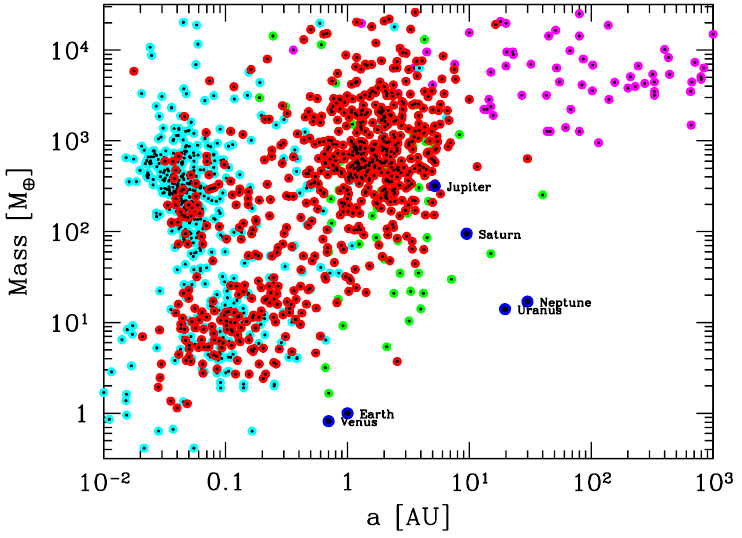
\includegraphics[width=0.9\textwidth]{obsMa}\label{fig:Maplot}
\caption{Da \cite{mordasini2018}.}
\end{figure}

\section{Popolazione esopianeti rilevati tramite RV}

Se l'asse z \'e lungo la linea di vista la posizione della stella \'e $z=r(t)\sin{i}\sin{(\omega+\nu)}$ e per la velocit\'a radiale:
\begin{align}
&v_r=\dot{z}=K[\cos{(\omega+\nu)}+e\cos{\omega}]\label{eq:vrsignal}\\
&K=\frac{2\pi}{P}\frac{a_*\sin{i}}{(1-e^2)\expy{1/2}}=(\frac{2\pi G}{P})\expy{1/3}\frac{M_p\sin{i}}{(M_p+M_*)\expy{2/3}}\frac{1}{(1-e^2)\expy{1/1}}
\end{align}
dove $K$ \'e la semi-ampiezza.

\begin{workout}[Simulated radialo detection limit]
Perrymann pg 34 fig 2.25 d
paragrafo detectability and selection effects pg 14 perryman
\end{workout}

\begin{workout}[Radial velocity: dtectability and selection effects (pg 14)]
fig 2.6,fig 2.18
\end{workout}


\begin{workout}[Distribuzioni elementi orbitali: periodo e massa]

La distribuzione di $M_p\sin{i}$ osservata \'e mostrata in figura \ref{fig:RVmpdistro}, la distribuzione di periodo orbitale \ref{fig:PdistroM30}/\ref{fig:Pdistrom30} perpianeti di massa maggiore/minore di $30\mearth{}$, la distribuzione dei pianeti in funzione della metallicit\'a stellare in \ref{fig:freqZstar}.

\begin{figure}[!ht]
\begin{subfigure}[b]{0.47\textwidth}
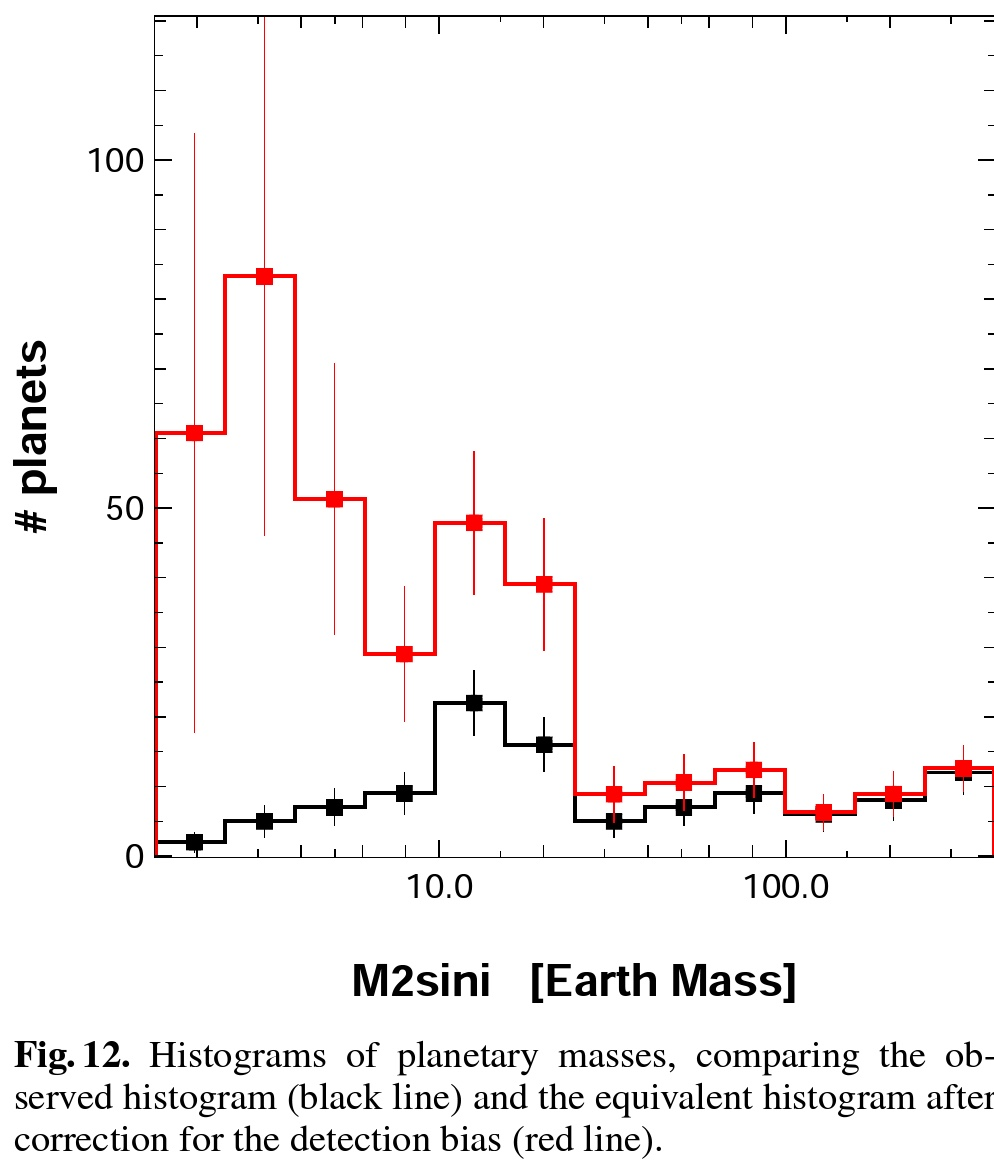
\includegraphics[width=0.9\textwidth]{freqvsM}
\caption{Diagramma $(M_p,a$ dei pianeti extrasolari osservati (The extrasolar planet encyclopedia -2017): evidenziati in rosso i pianeti rivelati tramite RV, celeste tramite transito, rosa tramite imaging e verde tramite microlensing. Da \cite{howard2012planet}.}\label{fig:Mdistro}
\end{subfigure}
~
\begin{subfigure}[b]{0.47\textwidth}
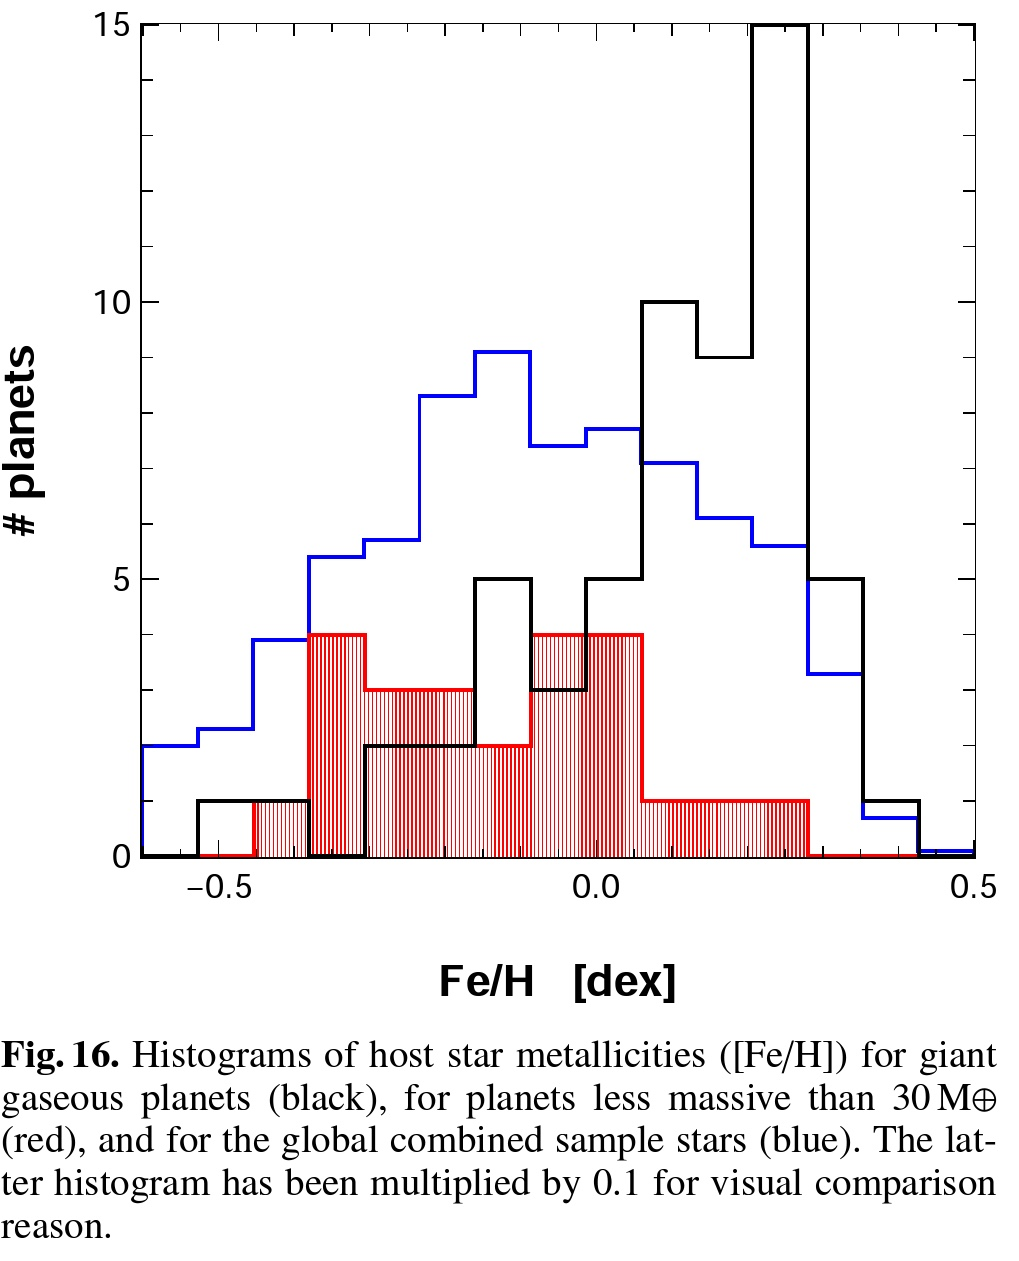
\includegraphics[width=0.9\textwidth]{PfreqvsFeH}\label{fig:freqZstar}
\caption{Da \cite{mayor2011harps}}
\end{subfigure}
\end{figure}

\begin{figure}[!ht]
\begin{subfigure}[b]{0.47\textwidth}
\centering
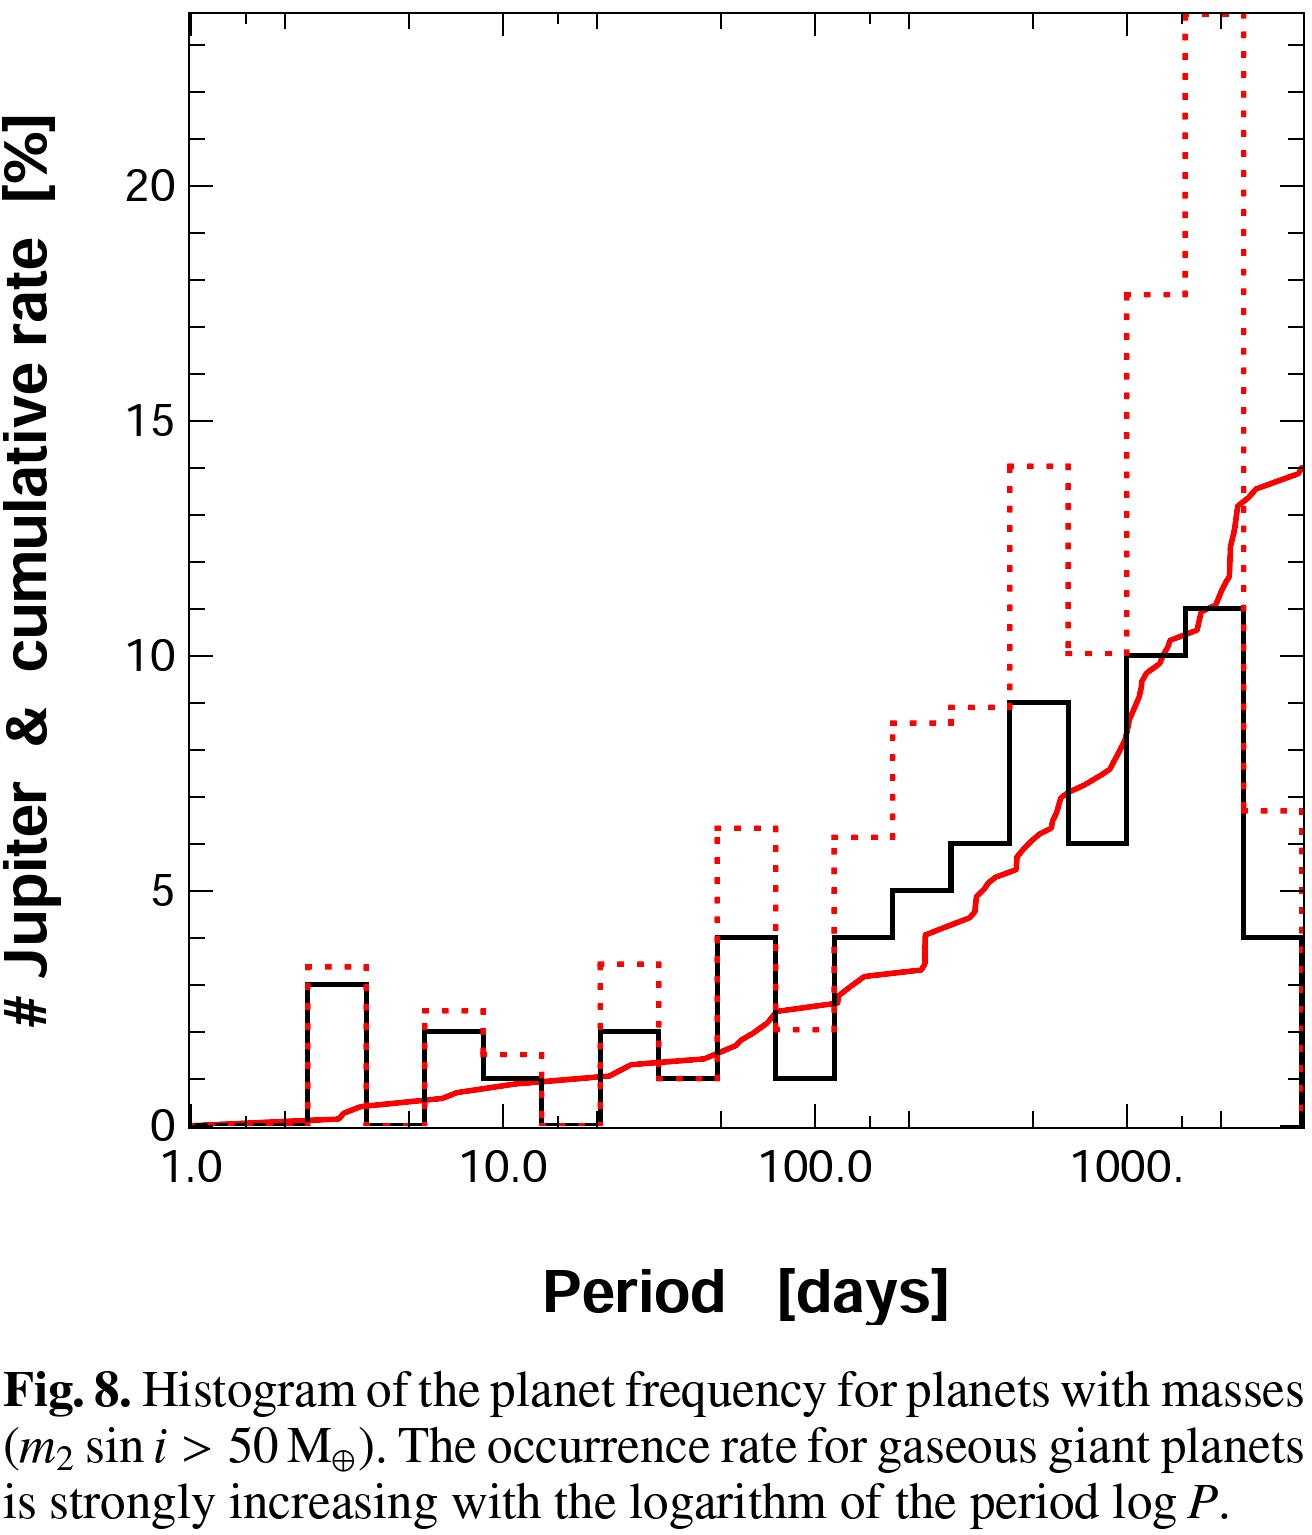
\includegraphics[width=0.9\textwidth]{freqvsPgiant}
\caption{Da \cite{mayor2011harps}}\label{fig:PdistroM30}
\end{subfigure}
~
\begin{subfigure}[b]{0.47\textwidth}
\centering
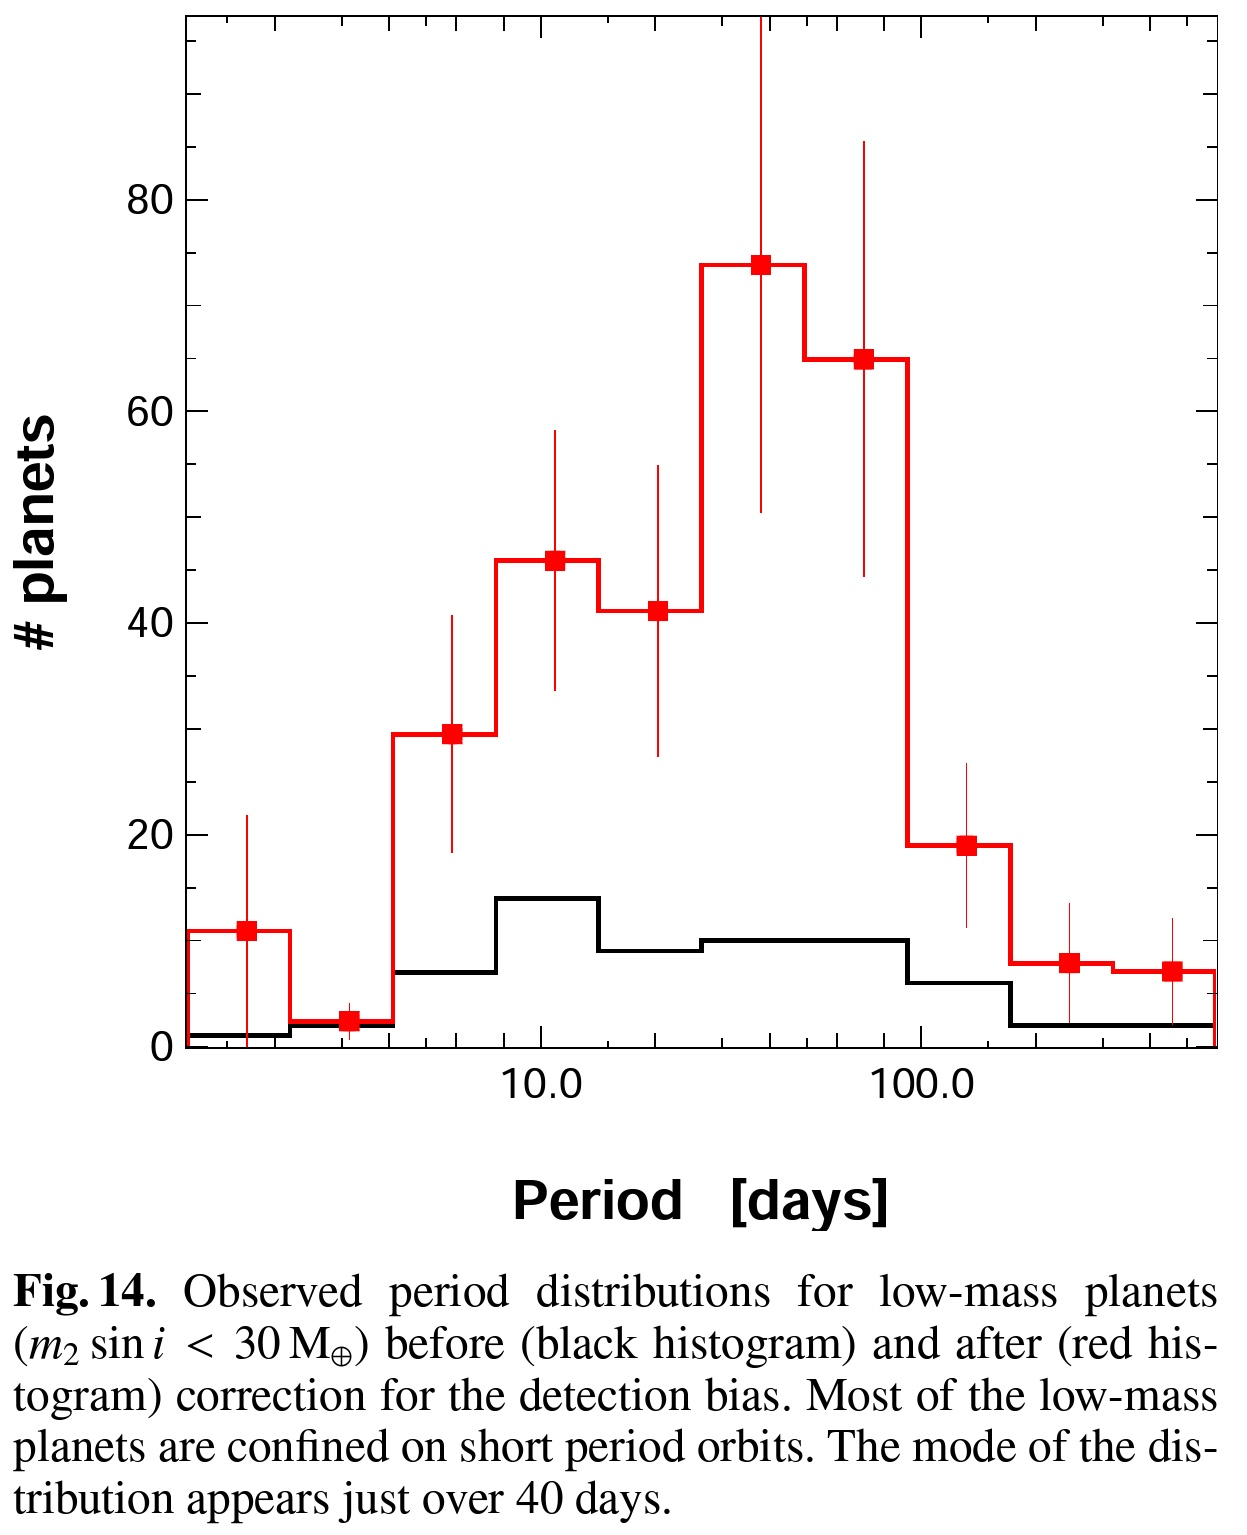
\includegraphics[width=0.9\textwidth]{freqvsPlowM}\label{fig:Pdistrom30}
\caption{Da \cite{mayor2011harps}}
\end{subfigure}
\end{figure}

\end{workout}

\begin{workout}[multplanet system: mean motion resonances, orbital spacing]
wright09: ten multiplanet sysytem and systematic
Winn, Fabricky 15
fig 2.30 pg 39 Perrymann
\end{workout}

%\begin{figure}[]
%\begin{subfigure}[b]{0.47\textwidth}
%\centering
%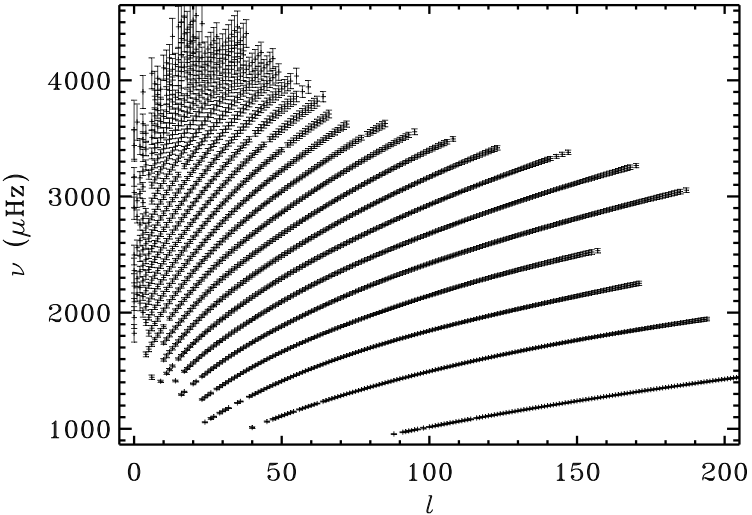
\includegraphics[keepaspectratio,width=0.95\textwidth]{midlmodes}
%\caption{I picchi della densit\'a spettrale si dispongono su creste in cui \'e concentrata la potenza in accordo al modello. Determinata usando i primi 144 giorni di osservazione di MDI con $l\leq300$. Da \cite{chr02helioseismology}.}\label{fig:midlmodes}
%\end{subfigure}
%~
%\begin{subfigure}[b]{0.5\textwidth}
%\centering
%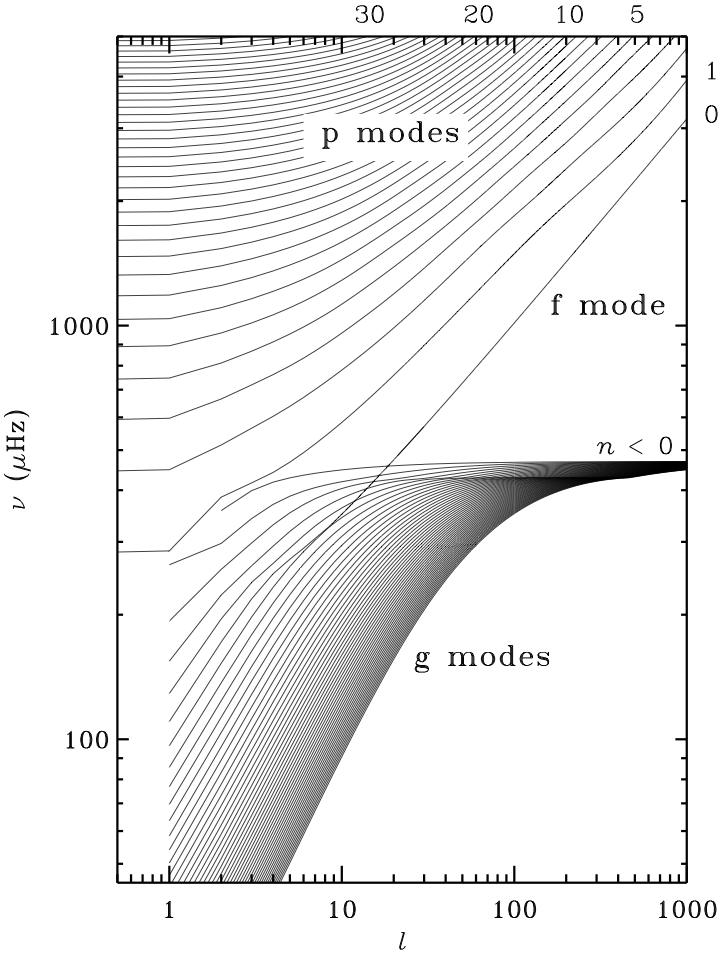
\includegraphics[keepaspectratio,width=0.95\textwidth]{nrmodesLAWE}
%\caption{Modi adiabatici calcolati sulla base di un modello solare. Da \cite{chr02helioseismology}.}\label{fig:nrmodesLAWE}
%\end{subfigure}
%\end{figure}

\begin{workout}[Radial velocity: keplerian observables (Appendice RV)]
La coordinata z della stella $z=r(t)\sin{i}\sin{(\omega+\nu)}$ e per la velocit\'a radiale
\begin{align}
&v_r=\dot{z}=K[\cos{(\omega+\nu)}+e\cos{\omega}]\label{eq:vrsignal}\\
&K=\frac{2\pi}{P}\frac{a_*\sin{i}}{(1-e^2)\expy{1/2}}=(\frac{2\pi G}{P})\expy{1/3}\frac{M_p\sin{i}}{(M_p+M_*)\expy{2/3}}\frac{1}{(1-e^2)\expy{1/1}}
\end{align}
Le osservabili $e$, $P$, $t_p$, $\omega$, $K=f(a,e,P,i)$ sono fittate per ogni pianeta.
La velocit\'a radiale della stella \'e
\begin{equation}
v_r(t)=K[\cos{(\omega+\nu(t)}+e\cos{\omega}]+\gamma+d(t-t_0)
\end{equation}
Per sistemi multipli consideriamo la sovrapposizione lineare di $n_p$ termini \eqref{eq:vrsignal}: viene sottratto il segnale Kepleriano dominante fino a che resta solo rumore.
\end{workout}

\begin{workout}[Radial velocity: keplerian observables (Appendix RV)]
La coordinata z della stella $z=r(t)\sin{i}\sin{(\omega+\nu)}$ e per la velocit\'a radiale
\begin{align}
&v_r=\dot{z}=K[\cos{(\omega+\nu)}+e\cos{\omega}]\label{eq:vrsignal}\\
&K=\frac{2\pi}{P}\frac{a_*\sin{i}}{(1-e^2)\expy{1/2}}=(\frac{2\pi G}{P})\expy{1/3}\frac{M_p\sin{i}}{(M_p+M_*)\expy{2/3}}\frac{1}{(1-e^2)\expy{1/1}}
\end{align}
Le osservabili $e$, $P$, $t_p$, $\omega$, $K=f(a,e,P,i)$ sono fittate per ogni pianeta.
La velocit\'a radiale della stella \'e
\begin{equation}
v_r(t)=K[\cos{(\omega+\nu(t)}+e\cos{\omega}]+\gamma+d(t-t_0)
\end{equation}
\end{workout}

Per sistemi multipli consideriamo la sovrapposizione lineare di $n_p$ termini \eqref{eq:vrsignal}: viene sottratto il segnale Kepleriano dominante fino a che resta solo rumore.

\begin{workout}[Radial velocity: dtectability and selection effects (pg 14)]
fig 2.6,fig 2.18
\end{workout}


\section{Popolazione esopianeti rilevati tramite transito}

Le osservabili sono la differenza di luminosit\'a durante il transito, la durata totale e di massima occultazione del transito, e il periodo: da questi \'e possibile ricavare $R_p$, a, i, $R_*$, e facendo uso della relazione massa raggio appropriata per la fase evolutiva della stella $M_*$

La probabilit\'a che l'orbita di un pianeta sia allineata con l'osservatore in maniera da avere un transito, per orbite circolari ed eccentriche, \'e:
\begin{align*}
&p=\frac{R_*}{a}=0.005(\frac{R_*}{\rsun{}})(\frac{a}{1AU})\expy{-1}\\
&p=(\frac{R_*\pm R_p}{a})(\frac{1}{1-e^2})
\end{align*}
La maggiore probabilit\'a \'e compensata approssimativamente dalla minore durata del transito.

\begin{workout}[Radial velocity: dectability and selection effects]
Considerando un numero totale di osservazioni $N_o$ durante il transito si hanno $N_t\approx N_o\frac{R_*}{\pi a}$; il rapport segnale rumore \'e $S/N=\sqrt{N_t}\frac{\delta}{\sigma}$, $\sigma$ precisione fotometrica, $\sigma\propto\frac{1}{\sqrt{N_{ph}}}\propto d$. Per fissato S/N e tipo stellare il numero di pianeti rivelati varia come
\begin{equation}
V_p*P\propto d^3*\frac{R_*}{a}\propto R_p^6/P\expy{\frac{5}{3}}
\end{equation}
\end{workout}


\begin{workout}[transit survey Kepler: coughlin 2016]
PLANETARY CANDIDATES OBSERVED BY KEPLER. VII. THE FIRST FULLY UNIFORM CATALOG BASED ON THE ENTIRE 48 MONTH DATASET (Q1–Q17 DR24
\end{workout}


\begin{workout}[transiti refs: osservabilie probabilit\'a di rilevamento]
pg103
pg 117, eccentric orbit pg 121-122
From space: presence of structure on stellar surface Perryman 3.4, Eriksson Lindegren 07; simulation of stellar jitter: Svensson Ludwig 05, Ludwig 06.
Probability of randomlyoriented planet on circular/eccentric orbit (Borucki Summers 84/Barnes 07, Burke 08,  Seagroves 03, Kane von Braun 08):
\end{workout}

\begin{workout}[Transiti: Propriet\'a dei pianeti a transito]
pg 143, fig 6.33, 6.34, 6.35
Mass-radius relation: chabrier 09
\end{workout}


\begin{workout}[Atmosphere and starting conditions]
fig 11.12
\end{workout}


\begin{workout}[M-R diagram]
orbital migration 10.8 Perryman, tidal effect 10.9, 
fig11.2, 11,4 (EOS), 11.7, 11.8 (M-R)
Ternary diagram 11.9, M-R realtion
Fig 6.33/34/35: mass radius realtion

pg 144: theoretical model - La posizione di un pianeta nel diagramma M-R fornisce indicazione della composizione
fig 6.35
\end{workout}


%\section{Struttura interna, composizione/diagramma $(M,R)$}
